\documentclass[11pt,a4paper]{ivoa}
\input tthdefs

\DeclareUnicodeCharacter{00B0}{$\deg$}
\DeclareUnicodeCharacter{00B5}{$\mu$}
\DeclareUnicodeCharacter{00B1}{$\pm$}

% epn-tap has some wide displays; give it a bit more room (at
% the expense of readability).
\usepackage[lmargin=2cm,rmargin=3cm]{geometry}
\usepackage{longtable}
\usepackage{todonotes}

\title{EPN-TAP: Publishing Solar System Data to the Virtual Observatory}

% see ivoatexDoc for what group names to use here
\ivoagroup{SSIG}

\author{Baptiste Cecconi}
\author{Stéphane Erard}
\author{Pierre Le Sidaner}
\author{Whoever Else}

\editor{Baptiste Cecconi}

% \previousversion[????URL????]{????Funny Label????}
\previousversion{This is the first public release}
       

\begin{document}
\begin{abstract}
???? Abstract ????
\end{abstract}


\section*{Acknowledgments}

???? Or remove the section header ????

\section*{Conformance-related definitions}

The words ``MUST'', ``SHALL'', ``SHOULD'', ``MAY'', ``RECOMMENDED'', and
``OPTIONAL'' (in upper or lower case) used in this document are to be
interpreted as described in IETF standard RFC2119 \citep{std:RFC2119}.

The \emph{Virtual Observatory (VO)} is a
general term for a collection of federated resources that can be used
to conduct astronomical research, education, and outreach.
The \href{http://www.ivoa.net}{International
Virtual Observatory Alliance (IVOA)} is a global
collaboration of separately funded projects to develop standards and
infrastructure that enable VO applications.


\section{Introduction}

???? Write something ????

\subsection{Role within the VO Architecture}

\begin{figure}[thb]
\centering

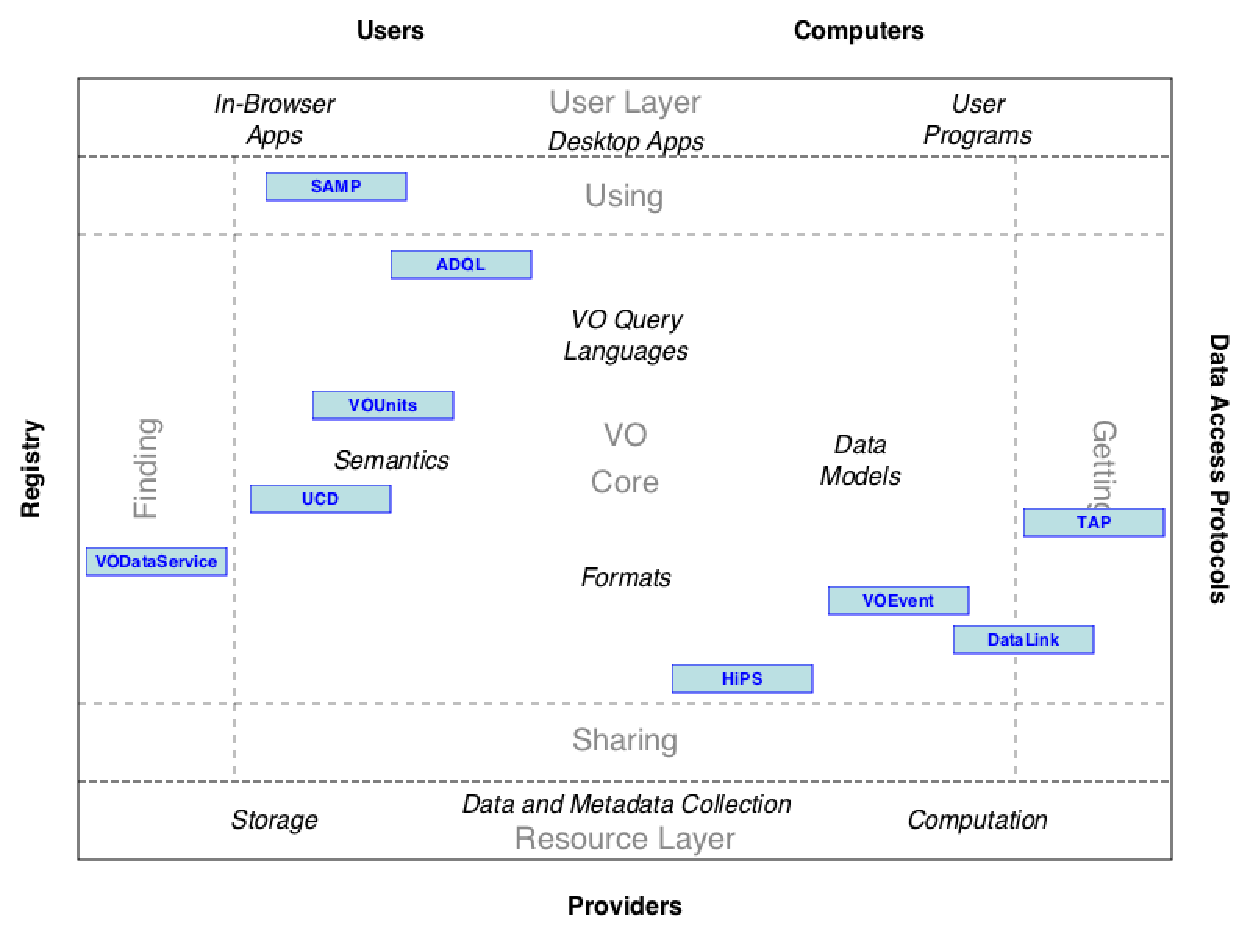
\includegraphics[width=0.9\textwidth]{role_diagram.pdf}
\caption{Architecture diagram for this document}
\label{fig:archdiag}
\end{figure}

Fig.~\ref{fig:archdiag} shows the role this document plays within the
IVOA architecture \citep{note:VOARCH}.


\clearpage % remove when there's enough page so the float doesn't get lost

\section{The EPN-TAP Table Structure}

% GENERATED: python parse_source.py columntable
\begingroup\small\begin{longtable}{p{3.5cm}p{0.5cm}p{1cm}p{1cm}p{7cm}p{3cm}}
\sptablerule
\textbf{Name}&\textbf{Req}&\textbf{Type}&\textbf{Unit}&\textbf{Description}&\textbf{UCD}\\\sptablerule\endfirsthead
\sptablerule
\textbf{Name}&\textbf{Req}&\textbf{Type}&\textbf{Unit}&\textbf{Description}&\textbf{UCD}\\\sptablerule\endhead
\multicolumn{6}{c}{\vrule width 0pt height 20pt depth 12pt \textbf{\textbf{EPNCore mandatory parameters}(Must be present, possibly empty)}}\\
granule\_uid&Y&Text&&Internal table row index.Unique ID in data service. &meta.id  meta.id;meta.dataset\\
granule\_gid&Y&Text&&Common to granules of same type&meta.id\\
obs\_id&Y&Text&&Associates granules derived from the same data &meta.id;obs \\
dataproduct\_type&Y&Text&&Organization of the data product, from enumerated list&meta.code.class\\
target\_name&&Text&&Standard IAU name of target (from a list related to target class), case sensitive.&meta.id;src\\
target\_class&Y&Text&&Type of target, from enumerated list&src.class\\
time\_min&&Double&d (date as JD)&Start time (in JD). UTC measured at time\_origin location (default is observer's frame)&time.start;obs\\
time\_max&&Double&d (date as JD)&Stop time (in JD). UTC measured at time\_origin location (default is observer's frame)&time.end;obs\\
time\_sampling\_step\_min&&Double&s&Min time sampling step&time.resolution;stat.min\\
time\_sampling\_step\_max&&Double&s&Max time sampling step&time.resolution;stat.max\\
time\_exp\_min&&Double&s&Min integration time&time.duration;obs.exposure;stat.min (\textbf{Deleted})







\\
time\_exp\_max&&Double&s&Max integration time&



time.duration;obs.exposure;stat.max











\\
spectral\_range\_min&&Double&Hz&Min spectral range (frequency)&em.freq;stat.min\\
spectral\_range\_max&&Double&Hz&Max spectral range (frequency)&em.freq;stat.max\\
spectral\_sampling\_step\_min&&Double&Hz&Min spectral sampling step&\emph{em.freq.step;stat.min} \\
spectral\_sampling\_step\_max&&Double&Hz&Max spectral sampling step&\emph{em.freq.step;stat.max }\\
spectral\_resolution\_min&&Double&&Min spectral resolution (resolving power)&spect.resolution;stat.min\\
spectral\_resolution\_max&&Double&&Max spectral resolution (resolving power)&spect.resolution;stat.max\\
c1min&&Double&(1)Longitude from 0. to 359.9999RA from 0. to 23.9999&Min of first coordinate&pos;stat.minpos.distance;stat.min (bof)or \emph{pos.radius;stat.min} (does not exist)  for spherical \& cylindricalpos.eq.ra;stat.min for celestial pos.bodyrc.lon;stat.min for bodypos.cartesian.x;stat.min for Cartesianpos.healpix for healpix (with 2 parameters?  - weird) - TBCempty ("") for none (and no unit)\\
c1max&&Double&(1)&Max of first coordinate&pos;stat.max, etc\\
c2min&&Double&(1)Latitude from -89.9999 to +89.9999&Min of second coordinate&pos;stat.minpos.angDistance;stat.minor pos.az.zd;stat.min (for zenithal distance) for spherical or pos.az.azi;stat.min (for azimuth)  for cylindricalpos.eq.dec;stat.min for celestial pos.bodyrc.lat;stat.min for bodypos.cartesian.y;stat.min for Cartesianempty ("") for none (and no unit)\\
c2max&&Double&(1)&Max of second coordinate&pos;stat.max, etc\\
c3min&&Double&(1)&Min of third coordinate&pos;stat.minpos.AngDistance;stat.min or pos.az.azi;stat.min (for azimuth)  for sphericalpos.distance;stat.min  for cylindricalpos.distance;stat.min for celestial pos.bodyrc.alt;stat.min for body? (from surface only, implicitly from reference level)orpos.distance;pos.bodyrc;stat.min for body (from center)?pos.cartesian.z;stat.min for Cartesian empty ("") for none (and no unit)\\
c3max&&Double&(1)&Max of third coordinate&pos;stat.max, etc\\
s\_region&&spoly&PgSphere spoly&ObsCore-like footprint for celestial, spherical, or body-fixed frames.&phys.outline;obs.field\\
c1\_resol\_min&&Double&(1)&Min resolution in first coordinate&pos.resolution;stat.min\emph{}\emph{}\emph{if linear} pos.angResolution;stat.min \emph{if angular}\\
c1\_resol\_max&&Double&(1)&Max resolution in first coordinate&pos.resolution;stat.max\emph{}\emph{}\emph{if linear} pos.angResolution;stat.max\emph{if angular}\\
c2\_resol\_min&&Double&(1)&Min resolution in second coordinate&pos.resolution;stat.min\emph{}\emph{if linear} \emph{pos.angResolution;stat.min }\emph{if angular}\\
c2\_resol\_max&&Double&(1)&Max resolution in second coordinate&pos.resolution;stat.max\emph{if linear} pos.angResolution;stat.max \emph{}\emph{if angular}\\
c3\_resol\_min&&Double&(1)&Min resolution in third coordinate&pos.resolution;stat.min\emph{if linear} pos.angResolution;stat.min \emph{if angular (spherical only)}\\
c3\_resol\_max&&Double&(1)&Max resolution in third coordinate&pos.resolution;stat.max\emph{if linear}  pos.angResolution;stat.min \emph{}\emph{if angular (spherical only)} \\
spatial\_frame\_type& Y&Text&(1)Use ``none'' if undefined&Flavor of coordinate system, defines the nature of coordinates. From enumerated list&meta.code.class;pos.frame\\
incidence\_min&&Double&deg&Min incidence angle (solar zenithal angle)& pos.incidenceAng;stat.min \\
incidence\_max&&Double&deg&Max incidence angle (solar zenithal angle)& pos.incidenceAng;stat.max \\
emergence\_min&&Double&deg&Min emergence angle& pos.emergenceAng;stat.min \\
emergence\_max&&Double&deg&Max emergence angle& pos.emergenceAng;stat.max\\
phase\_min&&Double&deg&Min phase angle&pos.phaseAng;stat.min\\
phase\_max&&Double&deg&Max phase angle&pos.phaseAng;stat.max\\
instrument\_host\_name&&Text&&Standard name of the observatory or spacecraft&meta.id;instr.obsty\\
instrument\_name&&Text&&Standard name of instrument&meta.id;instr\\
measurement\_type&&Text&&UCD(s) defining the data&meta.ucd\\
processing\_level&&Integer&&Use dataset-related value. If none defined, use simplified CODMAC calibration level&meta.calibLevel\\
creation\_date&Y&Timestamp&(ISO-8601 String)&Date of first entry of this granule&time.creation\\
modification\_date&Y&Timestamp&(ISO-8601 String)&Date of last modification&time.processing\\
release\_date&Y&Timestamp&(ISO-8601 String)&Start of public access period (set to creation\_date if no proprietary period)&time.release\\
service\_title&Y&Text&&Title of resource = schema name&meta.title\\
\multicolumn{6}{c}{\vrule width 0pt height 20pt depth 12pt \textbf{\textbf{Common optional parameters}}}\\
access\_url&&Text&&URL of the data file, case sensitive (additional files may be linked through datalink\_url). Can point to a script. If present, next 2 parameters must also be present.&meta.ref.url;meta.file\\
access\_format&&Text&(mime type\footnote{\url{https://voparis-confluence.obspm.fr/display/VES/Data+Formats+and+MIME+Types}} in lowercase)&File format type  &meta.code.mime\\
access\_estsize&&Integer&kbyte&Estimate file size in kbyte (with this spelling)&phys.size;meta.file\\
access\_md5&&Text&&MD5 Hash for the file when available (real file, not script)&\emph{ meta.checksum;meta.file}\\
thumbnail\_url&&Text&&URL of a thumbnail image with predefined size (png ~200 pix, for use in a client only)&meta.ref.url;meta.preview  \\
file\_name&&Text&&Name of the data file only, case sensitive&meta.id;meta.file\\
datalink\_url&&Text&(url)&Provides links to files or services on the server&meta.ref.url;meta.datalink\\
species&&Text&&Identifies a chemical species, \emph{case sensitive}&meta.id;phys.atmol\\
waveband&&Text&&Electro-magnetic band, from enumerated list&instr.bandpass\\
alt\_target\_name&&Text&can be a hash list&Provides alternative target name if more common&meta.id;src\\
target\_region&&Text&&Type of region or feature of interest&obs.field\\
feature\_name&&Text&&Secondary name (e.g. standard name of a region of interest)&obs.field \\
publisher&&Text&&Resource publisher&meta.curation\\
bib\_reference&&Text&&Bibcode preferred if available, doi, or other biblio id, URL...&meta.bib\\
internal\_reference&&Text&&List of granule\_uid(s) in the current service&meta.id.cross\\
external\_link&&Text&(url)&Link to a web page providing more details on the \emph{granule}.&meta.ref.url\\
spatial\_coordinate\_description&&Text&&ID of specific coordinate system and version / properties&meta.code.class;pos.frame\\
spatial\_origin&&Text&&Defines the frame origin&meta.ref;pos.frame\\
time\_origin&&Text&&Defines \emph{where} the time is measured (e. g., ground vs spacecraft)&meta.ref;time.scale\\
time\_scale&&Text&&Always UTC in \emph{data} services - from enumerated list&time.scale\\
subsolar\_longitude&&Double&deg&Sub-solar point longitude&pos.bodyrc.lon\\
subsolar\_latitude&&Double&deg&Sub-solar point latitude&pos.bodyrc.lat\\
subobserver\_longitude&&Double&deg&Sub-observer point longitude (sub-Earth for ground based observations)&pos.bodyrc.lon\\
subobserver\_latitude&&Double&deg&Sub-observer point latitude (sub-Earth for ground based observations)& pos.bodyrc.lat\\
ra&&Double&deg &Right ascension (not hour angle!)&pos.eq.ra;meta.main\\
dec&&Double&deg&Declination&pos.eq.dec;meta.main\\
radial\_distance\_min&&Double&km&Min distance from center (in body-fixed frame)&pos.distance;pos.bodyrc;stat.min\\
radial\_distance\_max&&Double&km&Max distance from center (in body-fixed frame)&pos.distance;pos.bodyrc;stat.max\\
altitude\_fromshape\_min&&Double&km&Min altitude above shape model / DTM (in body-fixed frame)&pos.bodyrc.alt;stat.min\\
altitude\_fromshape\_max&&Double&km&Max altitude above shape model / DTM (in body-fixed frame)&pos.bodyrc.alt;stat.max\\
solar\_longitude\_min&&Double&deg&Min Solar longitude Ls (location on orbit / season)&pos.ecliptic.lon;pos.heliocentric;stat.min  \\
solar\_longitude\_max&&Double&deg&Max Solar longitude Ls (location on orbit / season)&pos.ecliptic.lon;pos.heliocentric;stat.max \\
local\_time\_min&&Double&h&Min local time at observed region&time.period.rotation;time.phase;stat.min\\
local\_time\_max&&Double&h&Max local time at observed region&time.period.rotation;time.phase;stat.max \\
target\_distance\_min&&Double&km&Min observer-target distance&pos.distance;stat.min\\
target\_distance\_max&&Double&km&Max observer-target distance&pos.distance;stat.max\\
target\_time\_min&&Double&d&Min observing time in target frame &time.start;src\\
target\_time\_max&&Double&d&Max observing time in target frame&time.end;src\\
earth\_distance\_min&&Double&au&Min Earth-target distance&pos.distance;stat.min\\
earth\_distance\_max&&Double&au&Max Earth-target distance&pos.distance;stat.max\\
sun\_distance\_min&&Double&au&Min Sun-target distance&pos.distance;stat.min\\
sun\_distance\_max&&Double&au&Max Sun-target distance&pos.distance;stat.max\\
\multicolumn{6}{c}{\vrule width 0pt height 20pt depth 12pt \textbf{\textbf{Parameters from extensions}}}\\
obs\_mode&&Text&&Observing mode&meta.code;instr.setup\\
detector\_name&&Text&&Detector name&meta.id;instr.det\\
opt\_elem&&Text&&Optical element name&meta.id;instr.param\\
filter&&Text& &Identifies filter in use, typically for images.&meta.id;instr.filter\\
instrument\_type&&Text&&type of instrument&meta.id;instr\\
acquisition\_id&&Text&&ID of the data file/acquisition in the original archive&meta.id\\
proposal\_id&&Integer&&Proposal identifier&meta.id;obs.proposal\\
proposal\_pi&&text&&Proposal principal investigator&meta.id.PI;obs.proposal\\
proposal\_title&&Text&&Proposal title&meta.title;obs.proposal\\
campaign&&Text&&Name of the observational campaign&meta.id;meta.code\\
target\_description&&Text&&Original target keywords&meta.note;src\\
proposal\_target\_name&&Text&&target name as in proposal title&meta.note;obs.proposal\\
target\_apparent\_radius&&Double&?&Apparent radius of the target&phys.angSize;src\\
north\_pole\_position&&Double&deg&North pole position angle with respect to celestial north pole&pos.posAng\\
target\_primary\_hemisphere&&Text&&Primary observed hemisphere&meta.id;obs.field\\
target\_secondary\_hemisphere&&Text&&Secondary observed hemisphere&meta.id;obs.field\\
platesc&&Double&arcsec/pixel&spatial resolution per pixel or platescale (on sky only)&instr.scale\\
orientation&&Double&&Position angle of image y axis (on sky only)&pos.posAng\\
observer\_name&&Text&&Observer name&obs.observer;meta.main\\
observer\_institute&&Text&&Observer institute&meta.note;meta.main\\
observer\_id&&Integer&&Image observer's PVOL numeric identifier&meta.id.PI\\
observer\_code&&Text&&Image observer's PVOL username&meta.id.PI\\
observer\_country&&Text&&Image observer's country of residence&meta.note;obs.observer\\
observer\_lon&&Double&&Observer's approximate longitude&obs.observer;pos.earth.lon\\
observer\_lat&&Double&&Observer's approximate latitude&obs.observer;pos.earth.lat\\
mass&&Double&kg& Mass of object&phys.mass\\
sideral\_rotation\_period&&Double&h& Object rotation rate&time.period.rotation\\
mean\_radius&&Double&km&&phys.size.radius\\
equatorial\_radius&&Double&km&&phys.size.radius\\
polar\_radius&&Double&km&&phys.size.radius\\
diameter&&double&km&Target diameter, or equivalent diameter for binary objects&phys.size.diameter\\
semi\_major\_axis&&Double&au&&phys.size.smajAxis\\
inclination&&Double&&Orbit inclination&src.orbital.inclination\\
eccentricity&&Double&&Orbit eccentricity&src.orbital.eccentricity\\
long\_asc&&Double&deg&Longitude of ascending node, J2000.0&src.orbital.node\\
arg\_perihel&&Double&deg&Argument of Perihelion, J2000.0&src.orbital.periastron\\
mean\_anomaly&&Double&deg&Mean anomaly at the epoch&src.orbital.meanAnomaly\\
dynamical\_class&&Text&&Class of small body, from enumerated list&meta.code.class;src\\
dynamical\_type&&Text&&Subdivision of the class, from enumerated list&meta.code.class;src\\
taxonomy\_code&&Text&&Code for target taxonomy&src.class.color\\
magnitude&&Double&mag&Absolute magnitude. For small bodies, from HG magnitude system&phys.magAbs\\
flux&&Double&mJy&Target flux&phot.flux.density\\
albedo&&Double&&Target albedo&phys.albedo\\
map\_projection&&Text&&ID from enumerated list&\emph{pos.projection}\\
map\_height&&Double&pixel&Map size in px&phys.size\\
map\_width&&Double&pixel&Map size in px&phys.size\\
map\_scale&&Text&&Format TBD&pos.wcs.scale?\\
pixelscale\_min&&Double&km/pixel&Min pixel size on a surface&instr.scale;stat.min\\
pixelscale\_max&&Double&km/pixel&Max pixel size on a surface&instr.scale;stat.max\\
particle\_spectral\_type&&Text&&&meta.id;phys.particle\\
particle\_spectral\_range\_min&&Double&&&phys.energy;phys.particle;stat.minphys.mass;phys.particle;stat.min\\
particle\_spectral\_range\_max&&Double&&&phys.energy;phys.particle;stat.maxphys.mass;phys.particle;stat.max\\
particle\_spectral\_sampling\_step\_min&&Double&&&spect.resolution;phys.particle;stat.min \\
particle\_spectral\_sampling\_step\_max&&Double&&&spect.resolution;phys.particle;stat.max \\
particle\_spectral\_resolution\_min&&Double&&&spect.resolution;phys.particle;stat.min \\
particle\_spectral\_resolution\_max&&Double&&&spect.resolution;phys.particle;stat.max \\
original\_publisher&&Text&&Refers to the source of the data, especially in compilations of experimental data&meta.note;meta.main\\
producer\_name&&Text&&Data producer name, especially in compilations of experimental data&meta.note;meta.main\\
producer\_institute&&Text&&Data producer institute, especially in compilations of experimental data&meta.note;meta.main\\
sample\_id&&Text&&Provides a local ID in an existing catalogue (in addition to target\_name)&meta.id;src\\
sample\_classification&&Text&hash list&Information related to class, sub-class, species… (using standard names)&meta.note;phys.composition\\
sample\_desc&&Text&can be a hash list&Describes the sample, its origin, and possible preparation&meta.note\\
data\_calibration\_desc&&Text&can be a hash list&Provides information on post-processing &meta.note\\
setup\_desc&&Text&can be a hash list&Describes the experimental setup if needed - may include Aperture (size of sample measured), etc&meta.note\\
geometry\_type&&Text&can be a hash list&Type of observation, from enumerated list&meta.note;instr.setup\\
spectrum\_type&&Text&can be a hash list?&Type of spectral observation, from enumerated list TBD&meta.note;instr.setup\\
grain\_size\_min&&Double&µm&Min particle size in µm&phys.size;stat.min\\
grain\_size\_max&&Double&µm&Max particle size in µm&phys.size;stat.max\\
azimuth\_min&&Double&deg&Min azimuth angle for illumination&pos.azimuth;stat.min\\
azimuth\_max&&Double&deg&Max azimuth angle for illumination&pos.azimuth;stat.max\\
pressure&&Double&bar&Ambient pressure&phys.pressure\\
measurement\_atmosphere&&text&&Describes experimental conditions. ``vacuum'' for measurements under vacuum.&meta.note;phys.pressure\\
temperature&&Double&K&Ambient temperature&phys.temperature\\
event\_type&&Text&&Type of event from enumerated list (e. g., meteor\_shower, fireball, lunar\_flash, comet\_tail\_crossing…)&TBD\\
event\_status&&Text&&From enumerated list&TBD\\
event\_cite&&Text&&From enumerated list&TBD\\
\sptablerule
\end{longtable}
\endgroup

% /GENERATED




% GENERATED: python parse_source.py columndescription
% To ignore the following section, add 'Mandatory parameters' to IGNORED_SECTIONS
\subsection{Mandatory parameters}

\subsubsection{Granule references}

\paragraph{granule\_uid}

Unique granule ID in data service.

There can be only one file associated to a granule (plus possibly a thumbnail for quick-look purpose in a search interface).

\paragraph{granule\_gid}

Common to granules of same type (e.g. same map projection, or geometry data products) - think of it as a simple and convenient way to group or differentiate types of data.

When several files relate to the same data, this parameter helps distinguishing them. This will allow the user to select the type of data of interest. E. g., a service may provide links to calibrated images, plus raw data and ancillary information for every granule; these will share the same obs\_id, but will have different granule\_gid.

\paragraph{obs\_id}

Associates granules derived from the same data (e.g. various representations / processing levels). May be the ID of original observation.

\subsubsection{Data Description}

\paragraph{dataproduct\_type}

The dataproduct\_type parameter describes the high level scientific organization of the data product linked by the access\_url parameter (see below), or directly included in the table (in which case the value is 'ci' for catalogue\_item). EPNCore currently defines several types listed below. The data provider must select the type most adapted to his data. In complex situations (e. g., when a file contains several data products), several types can be used to describe the same granule (using a hash-list) — although using several granules to describe the file content may be a better solution.

In the epn\_core view these types are identified by a 2-characters ID, so that multivalued queries are unambiguous. Possible IDs are listed below with their meaning:

\begin{itemize}
\item \textbf{im }(= image): scalar field with two spatial axes, or association of several such fields, e.g., images with multiple color planes, from multichannel or filter cameras. Preview images (e.g. map with axis and caption) also belong here. Conversely, vectorial 2D fields are described as catalogue (see below).
\item \textbf{ma }(= map): scalar field / rasters with two spatial axes covering a large area and projected either on the sky or on a planetary body, associated to a map\_projection parameter (with a short enumerated list of possible values); each pixel is associated to 2D coordinates. This is mostly intended to identify complete coverages that can be used as reference basemaps. Does this require a secondary UCD notation (e.g., ;map)?
\item \textbf{sp }(= spectrum): measurements organized primarily along a spectral axis, e.g., radiance spectra. This includes spectral aggregates (series of related spectral segments with non-connected spectral ranges, e.g., from several channels of the same instrument, various orders from an échelle spectrometer, composite spectra, etc).
\item \textbf{ds }(= dynamic\_spectrum): consecutive spectral measurements through time, organized primarily as a time series. This typically implies successive spectra of the same target / field of view.
\item \textbf{sc }(= spectral\_cube): sets of spectral measurements with 1 or 2D spatial coverage, e.g., imaging spectroscopy. The choice between image and spectral\_cube is dictated by the characteristics of the instrument (which dimension is most resolved \& which dimensions are acquired simultaneously). The choice between dynamic\_spectrum and spectral\_cube is related to the uniformity of the field of view and by practices in the science field.
\item \textbf{pr }(= profile): scalar or vectorial measurements along 1 spatial dimension, e.g., atmospheric profiles, atmospheric paths, sub-surface profiles, traverses…
\item \textbf{vo }(= volume): measurements with 3 spatial dimensions, e.g., internal or atmospheric structures, including shells/shape models (3D surfaces).
\item \textbf{mo }(= movie): sets of chronological 2D spatial measurements (consecutive images)
\item \textbf{cu }(= cube): multidimensional data with 3 or more axes, e.g., all that is not described by other 3D data types such as spectral cube or volume. This is intended to accommodate unusual data with multiple dimensions.
\item \textbf{ts }(= time\_series): measurements organized primarily as a function of time (with exception of dynamical spectra and movies, i.e. usually a scalar quantity). Typical examples of time series include space-borne dust detector measurements, daily or seasonal curves measured at a given location (e.g. a lander), and light curves.
\item \textbf{ca }(= catalogue): applies to a single granule providing a catalog of object parameters, a list of features, a table in another TAP service, a list of events... ``Spatial vectors'' (e.g., vector information from a GIS, spatial footprints…) belong here. This is relevant, e. g., for collections of vectorial elements (e.g. crater contours or ROI definitions) which can be handled directly in a specialized environment such as a GIS. This includes maps of vectors, e.g., wind maps.
\item \textbf{ci }(= catalogue\_item): applies when the service itself provides a catalogue, with entries described as individual granules. The service can be, e. g., a list of asteroid properties or spectral lines. Catalogue\_item can be limited to scalar quantities (including strings), and possibly to a single element. This organization allows the user to search inside the catalogue from the TAP query interface.
\item \textbf{ev} (= event): introduces individual VOevents formatted according to IVOA standard (or possibly events with other formatting, TBC)
\end{itemize}

Usage:






\begin{verbatim}select * from epn\_core 
where dataproduct\_type like '\%im\%'\end{verbatim}




or 






\begin{verbatim}select * from epn\_core 
where ivo\_hashlist\_has(lower(dataproduct\_type), 'im') =1\end{verbatim}




will return only image data (the second syntax handles lists of values).

\paragraph{measurement\_type}

The measurement\_type parameter defines the physical quantities contained in the data, using UCDs. It relates to the reported quantity, not to the type of experiment. Therefore only UCD related to physical quantities can be used; e.g., phys.absorption;em.opt.I is eligible, while stellar\_occultation is not.

The provider must use the ``UCD1+'' list from IVOA as a reference, and should extend it only when necessary [RD8]: http://www.ivoa.net/documents/UCD1+/20180527/index.html\footnote{\url{http://www.ivoa.net/documents/UCD1+/20180527/index.html}}

The measurement\_type parameter is used to search data relevant to a certain field. Whenever several quantities are comprised in the granule, the measurement\_type parameter must therefore refer to all these quantities, including multiple UCDs if needed. Quantities derived from modeling/simulation are described by the regular UCD with ``;meta.modelled'' appended. 

Extra UCDs will be proposed/requested to IVOA. In the meantime, an extended list of UCDs will be made available in the EPN-DM document (in progress).

Examples:

\begin{itemize}
\item For images in general (i.e., actual measurements with a camera), the relevant UCD is obs.image (or obs.image;stat.uncalib if not calibrated).
\item For spectra phot.flux.density describes a \emph{flux} vector (irradiance), while radiance and reflectance are not really defined currently (the closest UCDs are phys.luminosity;phys.angArea;em.wl and phys.albedo). The associated spectral vector is described by UCDs em.wl, em.freq or em.energy, and the related error is described by stat.error;phot.flux.density (for flux).
\end{itemize}

\paragraph{processing\_level}

The processing\_level parameter is intended to provide the user with a quick evaluation of data ``usability''. When the original dataset uses a specific encoding of processing levels, this one should be used to meet expectations of the historical users; e. g., a service deriving from a telescopic archive will preferably use the processing levels from this archive. When no practice exists for a dataset, EPN-TAP uses a simplified version of CODMAC levels as described below.

Several classifications are in use in different contexts, as summarized in the table below.  EPNCore v2 uses the CODMAC / PDS3 levels but removes the intermediate calibration levels; this is equivalent to using the simplified PDS4 levels and maintaining a separated level for ancillary data \{reasons for this: level 4 is used in only 2 services by the end of 2016, and wrongly; this was also a strong suggestion from the reviewers of the 2014 paper\}. ``Partially calibrated'' datasets are in general considered as not calibrated, but this evaluation is up to the data provider depending on context. ``Ancillary'' data include all extra information documenting the measurements, in particular coordinates or geometry files. Several levels can be included in the same service (in particular calibrated and ancillary data) - although the publisher may decide to distribute various calibration levels in different data services. Only one value can be accommodated in this field, so the most advanced level (1-5) must be used whenever several levels are available in the same granule (TBD: use hash-list instead?).

Most EPN\_TAP data services are expected to include Calibrated or Derived data. Other values would therefore only flag associated products.



\begingroup\small\begin{inlinetable}
\begin{tabular}{lllllllp{0.35\textwidth}}
\sptablerule
EPN-TAP v2&CODMAC&PSA&NASA&PDS3&PDS4&ObsTAP&Description\\
\sptablerule

1 &1 (raw)&(0?)&&UDR&Telemetry&Level 0&Unprocessed Data Record (low-level encoding, e.g. telemetry from a spacecraft instrument. Normally available only to the original team)\\
2 &2 (edited)&1&0&EDR&Raw&Level 1&Experiment Data Record (often referred to as ``raw data'': decommutated, but still affected by instrumental effects)\\
3 &3 (calibrated)&2&1A&RDR&Calibrated&Level 2 (calibrated)&Reduced Data Record (``calibrated'' in physical units)\\
5&4 (resampled)&&1B&REFDR&Derived&~ Level 3 (enhanced)&Reformatted Data Record (mosaics or composite of several observing sessions, involving some level of data fusion)\\
5 &5 (derived)&3&2-5&DDR&Derived&~ Level 4 (analysis results)&Derived Data Record (result of data analysis, directly usable by other communities with no further processing)\\
6&6 (ancillary)&&&ANCDR&Derived&&Ancillary Data Record (extra data specifically supporting a data set, such as coordinates, geometry…) \\
\end{tabular}
\end{inlinetable}\endgroup

Notes:

\begin{itemize}
\item This table is a compilation of information from PSA, PDS4, \& ObsCore documents
\item The PDS3 column corresponds to the PDS3/PSA PRODUCT\_TYPE keyword
\item Descriptions are extracted from PSA documentation, with comments.
\end{itemize}

\subsubsection{Target description}

\paragraph{target\_name}

The target\_name element identifies a target by name or ID. The target may be any Solar System body, exoplanet, planetary sample, or meteorite, plus in some cases astronomical objects or spacecraft. Any other feature (craters, regions, atmospheric layers…) must be named using the optional feature\_name parameter (see 4.3.3). This parameter can be multivalued only to describe several targets related to a granule (e.g. with events). Alternative names of the same target cannot be listed here, but can be provided through the optional alt\_target\_name parameter. 

The best practice is to use the official designation of the target as defined by IAU [RD19]. This parameter is case sensitive (mixing lower/upper cases) and all values must use the standard spelling and case. Data providers must be aware that services which do not use the IAU designations might not be accessible by the clients. Conversely, users must be aware that some services containing data of interest might not be visible, if they do not use the recommended IAU nomenclature for planetary bodies. The SSODnet name resolver from IMCCE may help data providers (and users as well) to handle multiple denominations; it is available from the VESPA portal to support queries.

Concerning celestial objects (at fixed position, i. e., stars, galaxies…) the name should be identifiable through Simbad (http://simbad.u-strasbg.fr/simbad/\footnote{\url{http://simbad.u-strasbg.fr/simbad/}}).

Other best practices are listed below:

\begin{itemize}
\item The Exoplanet Encyclopedia provides a complete list of currently known extrasolar planets: http://exoplanet.eu/\footnote{\url{http://exoplanet.eu/index.php}}
\item Meteorite catalogs can be found here: http://www.nhm.ac.uk/research-curation/research/projects/metcat/search/indexsing.dsml\footnote{\url{http://www.nhm.ac.uk/research-curation/research/projects/metcat/search/indexsing.dsml}} and http://www.lpi.usra.edu/meteor/index.php\footnote{\url{http://www.lpi.usra.edu/meteor/index.php}}
\item The catalog of lunar samples is available here: http://www.lpi.usra.edu/lunar/samples/\footnote{\url{http://www.lpi.usra.edu/lunar/samples/}}
\item Other planetary samples are listed in topical web sites, e.g. samples from the Stardust mission are described here: http://curator.jsc.nasa.gov/stardust/catalog/\footnote{\url{http://curator.jsc.nasa.gov/stardust/catalog/}}
\item Asteroids: Usage is to use preferably name (if it exists) or principal designation (number is not used here, can be included in alt\_target\_name)
\item Calibration targets: Values can relate to existing names in a given archive (e.g., the PSA contains values such as bias, checkout, dark, flatfield, internal source…)
\end{itemize}

Usage:






\begin{verbatim}select * from epn\_core 
where target\_name like 'Ceres' or target\_name like 'Vesta' 
and target \_type like 'dwarf\_planet' or target\_class like 'asteroid'\end{verbatim}




Will return data only from 1 Ceres or 4 Vesta (see ADQL syntax). Complex queries may also include parentheses.

Example

1P is the official IAU designation for comet Halley.

\paragraph{target\_class}

The target\_class element identifies the type of a named target. A target is defined without ambiguity by a couple of parameters: target\_class and target\_name (although some targets may have no proper name).  EPNCore defines the possible values for target\_class:

\begin{itemize}
\item from IAU list [RD22]:\begin{itemize}
\item asteroid\\
\item dwarf\_planet
\item planet
\item satellite
\end{itemize}


\item extra values defined in EPNCore:\begin{itemize}
\item comet\\
\item exoplanet
\item interplanetary\_medium
\item ring
\item sample
\item sky
\item spacecraft
\item spacejunk
\item star
\item calibration
\end{itemize}


\end{itemize}

Usage:

\begin{itemize}
\item Any target has a unique target class.
\item ``interplanetary\_medium'' refers in particular to interplanetary dust.
\item ``sample'' refers to lunar or planetary samples, to meteorites, but also to terrestrial samples, e.g., in laboratory studies.
\item ``satellite'' stands for natural satellites only - other cases are handled though spacecraft or space junk.
\item ``star'' is used typically for calibration targets, and for the Sun.
\item ``sky'' may be used for other celestial bodies, usually referred to by their sky coordinates. It also includes the Interstellar Medium.
\item ``calibration'' is used for observations only related to instrument or signal calibration, including dark current, flat field, reference sample (in lab), etc.
\end{itemize}

\emph{Comment}: 

SsODNet uses ``Types'' of objects which are all included in EPN-TAP list: ``Asteroid'',``Spacecraft'',``Comet'',``Exoplanet'',``Spacejunk'',``Satellite'',``Planet'',``Dwarf Planet'',``Star'' Additional EPN-TAP classes are: interplanetary\_medium, ring, sample, sky, calibration \\

\subsubsection{Axes \\}

\paragraph{time (min/max)}

The time\_min and time\_max parameters provide the date and time of acquisition in the observer frame. 

In EPN-TAP, the time parameters are always provided in UTC and formatted in Julian days (expressed as a double precision float). Although ObsCore uses Modified JD, EPNCore uses standard JD to avoid ambiguity with time origin. With double precision floats, the accuracy is on the order of 1 ms, which is considered sufficient to identify data of interest (the initial accuracy is preserved in the data itself).

The two values min/max permit to handle long periods. Whenever acquisition time is a scalar (rather than an interval), both time\_min and time\_max must contain the same value in the table. There is no limiting value to this parameter.

Examples:

\begin{itemize}
\item Search data described by a time range:
\end{itemize}






\begin{verbatim}http://<server address>/tap/sync/request=doquery\&lang=adql\&query=select * from epn\_core where time\_min > '2455197.5' and time\_max < '2455927.5'\end{verbatim}




\begin{itemize}
\item Search data described by a start time parameter
\end{itemize}






\begin{verbatim}http://<server address>/tap/sync/request=doquery\&lang=adql \& query=select * from epn\_core where time\_min between '2455197.5' and '2455927.5'\end{verbatim}




Time range is normally provided in the observer frame (i.e., at the observer location), which is almost always the native time in the data. For instance, space-borne observations are usually documented with spacecraft on-board time, which is expected here (provided as JD, not as on-board clock timing). For other cases, the location where time is measured must be provided though the time\_origin parameter (see section 8).

To support space-borne vs ground-based campaigns, multiple spacecraft observations, or survey of periodic events, measurement times need to be corrected for light path. Whenever comparisons are potentially involved, the use of the target\_time\_min and target\_time\_max parameters is recommended in addition to time\_min and time\_max to simplify this kind of comparison.

Non-compulsory parameters may be used to accommodate additive, specially formatted time scales such as native on-board time (see section 8). The information of the time\_min and time\_max parameters is however greatly recommended for observations, as it is used by default to search datasets.

\paragraph{time\_sampling\_step (min/max)}

These parameters provide the sampling step for measurements of dynamical phenomena, and for computations. This is the time between 2 successive measurements or data, which is mostly relevant when the measurements are regularly spaced. This may also be used as an input parameter, e.g., for ephemeris computations. This parameter is intended to allow the user to search for time-resolved observations of dynamic phenomena.

\paragraph{time\_exp (min/max)}

These parameters correspond to the integration time (or exposure time) of measurements. It provides an estimate of the time resolution for dynamical phenomena, as well as an indication of relative S/N ratio inside a given dataset. This time is usually shorter than the time\_sampling\_step if both are present. It provides the overall integration time, i.e. individual exposure time x number of summed frames when relevant. 

\paragraph{spectral\_range (min/max)}

The spectral\_range parameters define the upper and lower bounds of the spectral domain of the data. As mentioned previously, this quantity is conventionally expressed on a frequency scale in Hertz.  The spectral range and associated parameters only apply to electromagnetic waves. See the optional parameters particle\_spectral\_* for particle energy or mass detection.

Since this is the standard parameter to identify a spectral location, it is recommended to fill it even for images obtained through a filter (central wvl ± FWHM/2, or even central wvl in both parameters, is enough for search purposes). 





\textbf{Conversions}




\begin{verbatim}with c = 2.99792458E8 (m/s)
spectral\_range\_min  = c*E6 /spectral\_range\_max\_micron
spectral\_range\_max  = c*E6 /spectral\_range\_min\_micron
(notice the inversion)\end{verbatim}




\paragraph{spectral\_sampling\_step (min/max)}

The spectral\_sampling\_step parameters provide the spectral separation between the centers of two adjacent filters or channels. Like all spectral\_* quantities, they are expressed on a frequency scale in Hz. 

These parameters are often most relevant for radio observations (long wavelengths / low frequency). They can also help distinguish between Nyqvist and sub-Nyqvist sampling rates (together with resolution).





\textbf{Conversions}




\begin{verbatim}with c = 2.99792458E8 (m/s)
df = c*1E6 dlam / lam^2 (from wavelength, with lam and dlam in micron)
df = c*1E3 dlam / lam^2 (same if dlam provided in nm)
df = c/1E-2 du (from wavenumber u in cm-1)\end{verbatim}




\paragraph{spectral\_resolution (min/max)}

The spectral\_resolution parameters actually provide the (dimensionless) resolving power: | lambda / Delta(lambda) | = | fq / Delta(fq) |   - to be updated in every service!

These parameters are mostly intended to provide an order of magnitude, e.g., to distinguish between Fourier spectrometers, grating spectrometers or filter cameras, or between observations related to surfaces or atmospheres. This is often most relevant for optical/infrared observations (short wavelengths / high frequency).





\textbf{Conversion}




\begin{verbatim}spectral\_resolution\_min  = abs( spectral\_range\_min\_micron / max(DeltaLambda) )
spectral\_resolution\_max  = abs( spectral\_range\_max\_micron / min(DeltaLambda) )\end{verbatim}




\\

\paragraph{c1 (min/max)}

\paragraph{c2 (min/max)}

\paragraph{c3 (min/max)}

These parameters provide up to three spatial coordinates of the measured target. The coordinates depend on the spatial frame type defined below. All services must handle three spatial coordinates, even if the third one is always set to NULL. Note that the c3 parameter is related to the observed area; the target distance (e. g., geocentric distance for ground based observations, or spacecraft distance) is introduced by the optional parameter ``target\_distance''.

In order to make uniform requests possible, spatial coordinates provided in the epn\_core view must be standardized. However, they can be provided in several systems types, as defined by the spatial\_frame\_type parameter.  The native coordinate system used with the dataset can be described by parameters spatial\_coordinate\_description and spatial\_origin. This is intended to provide this information prior to loading the data, especially when several coordinate systems are available in the same service. Descriptions for EPN-TAP are provided in [RD17]. Secondary coordinates can be introduced in the view using additional parameters, e.g., c1 and c2 providing central longitude and latitude of a planetary disk, and extra RA / DEC columns providing location on the sky at this moment.

\paragraph{c1\_resol (min/max)}

\paragraph{c2\_resol (min/max)}

\paragraph{c3\_resol (min/max)}

These parameters provide a simple estimate of resolution, either the FWHM of the PFS on the sky (in degrees), or the pixel size on a surface (in m), depending on spatial\_frame\_type. The client front-end may propose more appropriate units to the user, depending on context (e.g., angular resolution in mas, distance in m…).

\paragraph{spatial\_frame\_type}

Provides the "flavor" of the coordinate system, which defines the nature of the spatial coordinates (c1,c2,c3) in the epn\_core view and queries, and the way they are defined. This may be different from the coordinate system associated to / included in the data themselves. A value is required (use ``none'' if not applicable, ``body'' may also be OK in most cases). The possible types are described below:

\begin{itemize}
\item \textbf{celestial}: 2D angles on the sky, i. e. , right ascension c1 and declination c2 + possibly heliocentric distance in c3 – although this is a special case of spherical frame, the order and conventions are different. Earth distance may be provided as target\_distance whenever relevant (ground-based observations). Assumes ICRS coordinates; right ascension is provided in degrees.
\item \textbf{body:} 2D angles in body-fixed frame: longitude c1 and latitude c2 + possibly altitude (above a reference surface) as c3. \emph{(c3 is expected to only provide an order of magnitude in general, not to be a fine search parameter)}\\Planetocentric system with eastward longitudes in the range (0,360)° is expected. Current IAU frame is assumed, in particular for definition of  prime meridian. IAU 2009 planetocentric convention [RD12] applies, in particular eastward longitudes and a north pole located on the north side of the invariant plane of the Solar System for planets and satellites (see [RD12] for small bodies, and Annex A for details). \emph{ }\\\emph{The spatial\_coordinate\_description and spatial\_origin attributes allow the data provider to indicate different conventions, e. g., to indicate a planetographic frame, or to use altitude above a reference surface as the third coordinate. It is stressed however that using other frames will make comparisons between datasets more difficult.}\begin{itemize}
\item \emph{No, that would preclude uniform queries. These 2 param have to relate to the coordinates provided with the data.}
\item Two other parameters are available to provide other vertical scales, see below (radial\_distance and altitude\_fromshape). 
\item Planetary interiors have C3 <0 
\item Planetocentric rotating frames are defined as spherical (TBC)
\end{itemize}


\item \textbf{cartesian:} (x,y,z) as (c1,c2,c3). This includes spatial coordinates given in pixels.
\item \textbf{spherical:} (r, theta, phi) as (c1,c2,c3), as defined in ISO standard \footnote{\url{https://en.wikipedia.org/wiki/ISO\_80000-2}}80000-2:2009\footnote{\url{https://en.wikipedia.org/wiki/ISO\_80000-2}}; r = radius; theta = zenith angle/colatitude/inclination; phi = azimuth (E longitude). Angles are provided in degrees. When related to the sky or to a solid body, ``celestial'' (with RA/Dec) or ``body'' (with longitude/latitude) coordinates must be used instead.
\item \textbf{cylindrical:} (r, theta, z) as (c1,c2,c3); r = radius; theta = azimuth; z = height. The angle is provided in degrees.
\item \textbf{none:} to be used when no spatial frame is defined for the dataset. This is intended to prevent useless searches when space coordinates are not defined (a non-zero value is required by the mixin).\begin{itemize}
\item \emph{spatial\_origin} used to indicate center of frame ?
\item \emph{Not used in the view (only possible in the data) ?}
\end{itemize}


\item \textbf{healpix:} TBC (Nside and pixel\#? Should also specify or assume ordering (nested/ring) ) - TBC, wait for IVOA decision.
\end{itemize}

This parameter, although related to the specific coordinate system in use, is mostly intended to identify the nature of the coordinates handled by the service (e. g., angles versus distances). This parameter is provided as a column of the epn\_core view, to ensure it can be queried through the basic TAP mechanism. Although it will in general remain constant along the table for simple services, this parameter can vary from granule to granule and a value must therefore be provided in any query that includes spatial coordinates. Whenever additional coordinates are provided, they must be stored in extra columns of the table. If several different frames are mixed to provide the main coordinates, the use of different granule\_gid may help clarify the situation. At any rate, easy access to the data must be considered during the design of the service. \emph{Ranges and specific definitions vary with the actual frame in use, and are discussed in Appendix A. - Only applies to the system provided in the data?} 

\paragraph{incidence\_angle (min/max)}

The incidence angle parameters define the upper and lower bounds of the incidence angle variation in the data (also known as Solar Zenith Angle). This is always indicated in decimal degrees, and may range from 0 to 90° (with 0° indicating the normal to the surface). Incidence and emergence angles may be counted relative to the normal of the ellipsoid model, or to the local normal (e. g., using a 3D shape model). In case the two systems are included in the data, these keywords introduce the values relative to the ellipsoid (local values may be available through non-compulsory parameters).

\paragraph{emergence\_angle (min/max)}

The emergence angle parameters define the upper and lower bounds of the emergence angle variation in the data (viewing angle). This is always indicated in decimal degrees, and may range from 0 to 90° (with 0° indicating the normal to the surface). Incidence and emergence angles may be counted relative to the normal of the ellipsoid model, or to the local normal (e. g., using a 3D shape model). In case the two systems are included in the data, these keywords introduce the values relative to the ellipsoid (local values may be available through non-compulsory parameters).

\paragraph{phase\_angle (min/max)}

The phase angle parameters define the upper and lower bounds of the phase angle variation in the data (scattering angle - 180°, or angle light source-target-observer). This is always indicated in decimal degrees, and may range from -180 to 180° (with 0° corresponding to opposition, i. e., light source in the back of the observer). Negative values may refer, e. g., to geometry before opposition, depending on context. Phase (\emph{phi}), incidence and emergence are partly related:






\begin{verbatim}abs(i - e) < phi < i + e\end{verbatim}




If the azimuth angle \emph{a} is provided instead of the phase angle, the latter can be derived from knowledge of the three angles:






\begin{verbatim}cos phi = cos i cos e + cos a sin i sin e\end{verbatim}




\paragraph{s\_region}

Another mandatory parameter provides additional information about axes coverage.

This parameter introduces a footprint for spatially extended data products in 2D, most notably on the sky (using RA, Dec) or on planetary surfaces (using E longitude, latitude). This is a single parameter with no min/max declinations. It must contain a PgSphere spoly variable with syntax: '\{(lon1,lat1), (lon2,lat2), … \}' (with no quotes) where (lon1,lat1) = (10.d, 5d), character d included (for degrees). Pairs (lon1,lat1) must sample the dataproduct contour in sequence, provided in direct (counter-clockwise) sense. The result of the query is an STC-S string (as in ObsCore; currently retrained to polygons).\\

In addition, the resource descriptor (q.rd for DaCHS) must contain the line (for body coordinates):






\begin{verbatim}<stc>  Polygon UNKNOWNFrame [s\_region] </stc>\end{verbatim}




Open issue: this work directly in celestial coordinates, using ICRS as POLYGON value. On a planetary body, frame UNKNOWNFrame must be used. The difficulty is that W longitudes are assumed in this case. To be discussed at IVOA. The recommendation is to build s\_region contours using W longitudes for the time being, but this will change in the future.

\subsubsection{Data origin}

\paragraph{instrument\_host\_name}

This parameter provides the name of the observatory or spacecraft that performed the measurements. The best practice is to use names from the lists indicated below. A list of host names must be provided for integrated data sets. For ground-based observations, the reference is the list of IAU observatory codes: http://www.minorplanetcenter.net/iau/lists/ObsCodesF.html\footnote{\url{http://www.minorplanetcenter.net/iau/lists/ObsCodesF.html}}. However, this list is not intended to include all ground-based observatories, and a complement still needs to be identified (including e. g. radio-telescopes). A reasonably complete list of radio-telescopes is available here: http://en.wikipedia.org/wiki/List\_of\_radio\_telescopes\footnote{\url{http://en.wikipedia.org/wiki/List\_of\_radio\_telescopes}}. The WiseRep list also provides a  database of telescopes and instruments: https://wiserep.weizmann.ac.il/aux/telescopes\footnote{\url{https://wiserep.weizmann.ac.il/aux/telescopes}}, https://wiserep.weizmann.ac.il/aux/instruments\footnote{\url{https://wiserep.weizmann.ac.il/aux/instruments}}. 

Other open Q:

\begin{itemize}
\item are IAU ID eligible?
\item granularity is very heterogeneous (e.g., one single entry for Paranal or Mauna Kea, but many for Siding Spring).
\end{itemize}

Some entry related to obs programs (New Horizon KBO search from various sites)

Concerning space-borne data, the most complete list of international planetary missions and orbital observatories is found here (included in a complete list of space missions with ID): http://nssdc.gsfc.nasa.gov/nmc/\footnote{\url{http://nssdc.gsfc.nasa.gov/nmc/}}. Planetary missions are also listed here: http://nssdc.gsfc.nasa.gov/planetary/chronology.html\footnote{\url{http://nssdc.gsfc.nasa.gov/planetary/chronology.html}}. Alternatively, the PDS dictionary defines values for many mission names: http://pds.nasa.gov/tools/dictionary.shtml\footnote{\url{http://pds.nasa.gov/tools/dictionary.shtml}}. Other mission names are supported by the SPICE system, but only as ID codes: http://www-int.stsci.edu/~sontag/spicedocs/req/naif\_ids.html\footnote{\url{http://www-int.stsci.edu/\%7Esontag/spicedocs/req/naif\_ids.html}} (TBC – Spice is unambiguous but only uses IDs, PDS values are explicit but somewhat arbitrary). In the epn\_core view, the acronym is preferred to the full name to avoid long strings and related errors. Both values can be provided (e.g., HST + Hubble Space Telescope).

\paragraph{instrument\_name}

Identifies the instrument(s) that acquired the data. A list of instruments must be provided for integrated datasets. Service providers are invited to include multiple values for instrument name, e.g., complete name \& usual acronym. This will allow queries on either ``VISIBLE AND INFRARED THERMAL IMAGING SPECTROMETER'' or ``VIRTIS'' to produce the same reply. They must be separated by the \# character to be queried.

\emph{\emph{Example:}}






\begin{verbatim}VISIBLE AND INFRARED THERMAL IMAGING SPECTROMETER\#VIRTIS\end{verbatim}




Concerning space-borne data, the most complete list of international planetary missions and orbital observatories is found here: http://nssdc.gsfc.nasa.gov/nmc/\footnote{\url{http://nssdc.gsfc.nasa.gov/nmc/}}

Instruments on board planetary missions in particular are listed here: http://nssdc.gsfc.nasa.gov/nmc/experimentSearch.do\footnote{\url{http://nssdc.gsfc.nasa.gov/nmc/experimentSearch.do}}

\subsubsection{Granule call-back info}

\paragraph{service\_title}

Provides an acronym for the service/table title. This is used to refer to the service providing the data, therefore this must be identical to the name of the schema and must be constant in the view.\\When designing the service, care should be taken to use a schema name not already ascribed to another EPN-TAP service - must be unique on the provider side in any case.

\paragraph{creation\_date}

Provide the date when the granule was introduced

\paragraph{modification\_date}

Provide the date when the granule was last updated (intended to speed up mirroring between sites)

\paragraph{release\_date}

Provide the date when the granule becomes public (intended to preserve proprietary period, usage TBD)

% To ignore the following section, add 'Optional parameters' to IGNORED_SECTIONS
\subsection{Optional parameters}

\subsubsection{Data Access Reference}

\paragraph{access\_url}

The data of interest are often stored in a file, not in the table itself. In this very usual case, the access\_url parameter provides a complete path to the data products on the network, so that they are accessible for download by plotting or processing tools. All URLs in the epn\_core view are case sensitive and must provide an actual and unique link. The link may be a call to a web service (e.g., CRISM service) or the output of a script on the server (e.g. Titan atmospheric profiles service); in both cases the link must include the adequate arguments. In any case, this parameter must link to the actual data, not to a file of metadata nor a document. Datalinks (which typically open a page with either a list of links or an input interface for parameters) can be used for this purpose, and must be provided via the datalink\_url parameter. \\Whenever the data consists in a few scalar fields, this parameter may be replaced by parameters providing the data itself  in the table, which makes them searchable (e.g. mass, in a table providing the masses of Solar System bodies).

\paragraph{access\_format}

Access\_format provides the format of the data file linked through the access\_url parameter. \\The data may be stored in their native format, and no format conversion is required to set up an EPN-TAP service. This field can therefore include reference to unusual formats, although those may not be handled by plotting tools but only in a specific environment. Consistently with ObsCore, possible values are MIME-types written in lower cases and are listed on this page: Data Formats and MIME Types\footnote{\url{/display/VES/Data+Formats+and+MIME+Types}}.

\paragraph{access\_estsize}

The access\_estsize field provides an order of magnitude (in kilobytes) of the file available via the corresponding URL. It is intended to provide an indication that can help to tune download functionalities in an application, depending on data volume and transfer bit rate.

\\

\textbf{• Other parameters may be used to describe the data files:}

\paragraph{thumbnail\_url}

The thumbnail\_url parameter contains the URL of a reduced version of the data product used for quick-look purpose (e.g., a small jpeg image, typically 200x200 pixels). This may be handy in the case of big data files or unusual data formats, to facilitate data selection by the user. The EPN-TAP client uses this thumbnail for on-line quick-look, which therefore provides important added value to a service. Preferred formats include jpeg and png, which are handled easily by a basic viewer. Larger or more elaborate previews can be provided as independent granules and identified via a granule\_gid different from that of the data. All URLs in the epn\_core view are case sensitive and must provide an actual link.

\paragraph{file\_name}

The file\_name parameter introduces the name of the \emph{data} file, with extension but no path information. In many data services, the file name encodes the most relevant metadata and may be a very handy access mechanism for specialists. In services providing sets of files in a complicated directory tree (e.g., related to a spacecraft operation plan), the file\_name parameter is a handy key to perform automatic operations such as mirroring, pipeline processing, etc - a web service is available to retrieve a file from the file\_name parameter in any EPN-TAP service (File grabbing interface\footnote{\url{/display/VES/File+grabbing+interface}}). Its use is therefore always recommended when data are provided in separated files, i. e., not included in the table.\\All file\_name values in the epn\_core view are case sensitive and must reflect the filename of the product provided through access\_url; for instance, if this is a link to script converting an ascii file to VOTable, file\_name must refer to the outcome of this script, in this case the VOTable.

\paragraph{access\_md5}

This parameter introduces a MD5 Hash for the file when available (link to a real file), to be used as a checksum.\\

\paragraph{accref}

Not an EPN-TAP parameter, but apparently used to introduce an URL with datalink in TAP / DaCHS (present in epncore2 mixin) - really? Also generated automatically in q.rd when using the localfile mixin (when accessing data files located on the DaCHS server itself). See with developers for use in TOPCAT and VESPA portal. May also be required to handle proprietary periods, TBC. \\

\paragraph{datalink\_url}

This parameter is used to provide extra accesses through a datalink/SODA interface. It can either provide a table of hard links (dlmeta) or a dialogue to setup input values and call a web service (dlget). Input values can be retrieved from the current granule; if several EPN-TAP parameters need to be passed, they must be concatenated in an extra parameter in the table (often called \textbf{ds\_id}).

\subsubsection{Supplementary descriptions\\}

\paragraph{bib\_reference}

The bib\_reference parameter introduces an individual bibliographic reference at granule level. This may be required to provide the origin of the data, e. g., if the resource is a compilation of data from various origins. This is best provided as a bibcode (as used e. g. by ADS) or as a DOI.  A generic regular expression for bibcode (from IPDA discussions) is: [0-9]\{4\}[A-Za-z0-9$\backslash$\&$\backslash$.]\{5\}[A-Za-z0-9$\backslash$.]\{9\}[A-Z$\backslash$.] 

See http://adsabs.github.io/help/actions/bibcode\footnote{\url{http://adsabs.github.io/help/actions/bibcode}}

\paragraph{publisher}

Specifies the publisher of the \emph{data service} (not necessarily at the origin of the data). Currently a free format string.\\

\paragraph{internal\_reference}

The internal\_reference parameter can be used to identify granules (or sets of granules) intimately related to the current one. E.g., in a service containing both observations and results of analysis of observation sets, internal\_reference can be used to provide the set of observations used to compute a result. This contains a list of granule\_uid in the same service.\\This is specifically intended to provide internal references in services which would otherwise need to be split in several tables, and must not be used in more usual cases. 

\paragraph{external\_link}

The external\_link parameter can be used to provide extra information that does not fit easily in the view, and is intended for human reading only. This may be an extended discussion about a granule on a web site, which may include images, tables, or other documents. For instance, the individual planet pages of the Encyclopedia of exoplanets can be linked with this parameter. This parameter must contain a single URL.\\

\paragraph{species}

The species parameter introduces the chemical species of interest in simple data services. The formatting is very basic and simply uses the standard formula in ascii, e. g., H2O for water, CO2 for carbon dioxide or Fe for iron. This is the only query parameter that is provided in case sensitive form, using the standard chemical notation. This format can only accommodate atoms and simple molecular species, and does not support isotopic variations.  

An example application is related to atmospheric composition: a table providing the vertical abundances of many gaseous species with altitude. All columns are abundances and are described by the same measurement\_type parameter. Only the use of the ``species'' parameter (together with the column name itself) allows identifying the various species and accessing the requested information. If the data contain one column per species, it is recommended to also include the species in the column name (e.g., H2O\_abundance). 

If more elaborated compositional information must be included, the use of another parameter providing InChiKeys is recommended - TBC (inChiKey only related to molecule, including isotopes, but not physical state / phase; does not include \#)\\

\paragraph{filter}

This parameter introduces the standard name of a filter used during measurements. This is reserved for filters in imaging mode (no grating/grism \#, etc). There is no predefined list, because of the large variety of possible denominations, but the best practice is to use a short and accurate ID. 

This is intended to document the results of a search, rather than a search parameter. Therefore, it is recommended to also fill the spectral\_range\_min/max parameters to describe filter imaging - this is the only way to make filter imaging easily searchable.

\paragraph{alt\_target\_name}

This parameter introduces an alternative name of the target, especially when it is more usual than the official IAU one (e.g., Halley vs 1P).

Another possible usage is to store here a list of all alternative names of the target (e.g., for asteroids: name, number, principal and provisional designations).

\paragraph{feature\_name}

The feature\_name parameter introduces a supplementary name to provide more details about the observed target. It is intended in particular to accommodate a local name (crater, surface feature, region name…) whereas target\_name is reserved to describe the whole body (Mars, Moon, Ceres…). The best practice is to use the official features name defined by IAU [RD20] when relevant

The target\_region parameter (see below) also provides additional information on the target, but is aimed at indicating the global scope of a database (e.g., atmospheric layer, internal structure…).

\paragraph{target\_region}

This parameter optionally identifies the region of interest for the resource, in complement to target\_name. This parameter only introduces generic regions, not specific local names, which must be handled using the feature\_name parameter (see examples above).

The best practice is to take the values from standard sources:

\begin{itemize}
\item IVOA thesaurus: http://www.ivoa.net/rdf/Vocabularies/vocabularies-20091007/IVOAT/\footnote{\url{http://www.ivoa.net/rdf/Vocabularies/vocabularies-20091007/IVOAT/}}
\item IAU thesaurus http://www.mso.anu.edu.au/library/thesaurus/\footnote{\url{http://www.mso.anu.edu.au/library/thesaurus/}}\\+ another version: http://www.vocabularyserver.com/trex/en/\footnote{\url{http://www.vocabularyserver.com/trex/en/}}\\The latter seems more recent and more complete (although the interface is not practical)
\item Spase dictionary http://www.spase-group.org/\footnote{\url{http://www.spase-group.org/}}\\Example: \\\emph{``atmosphere'', ``surface'', ``ionosphere''}\\The same sources are used for the declaration file in the registry.
\end{itemize}

\subsubsection{Description of coordinate frame}

\paragraph{Spatial\_coordinate\_description}

\paragraph{Spatial\_origin}

These two parameters provide description of the spatial frame(s) in use, as introduced by the spatial\_frame\_type parameter. This is mostly relevant when this parameter is constant throughout the service. Possible values are detailed in [RD17], which is partly adapted from STC [RD13].

Spatial\_origin may be used to distinguish between altitude and distance from center when body coordinates are in use - TBC.

Examples (TBC)






\begin{verbatim}BODY, Mars\_IAU2000, ICRS
Geocenter \end{verbatim}




\paragraph{time\_origin}

This attribute states where the time is measured, and is expected to remain constant throughout the service. This knowledge is required to cross-correlate event-based observations, in particular to indicate light-path differences. It applies to the time\_min and time\_max parameters (target\_time always refers to the target in the FoV). If this parameter is not informed, time is expected to be provided in the observer frame. Possible values for time\_origin are:






\begin{verbatim}Earth, (solar system bodies), (spacecraft)\end{verbatim}




\paragraph{time\_scale}

Always UTC in \emph{data} services (may be relaxed in computational services such as ephemeris) — from enumerated list.

\subsubsection{Target configuration \& observing geometry}

\paragraph{solar\_longitude (min/max)}

Solar longitude (a.k.a. heliocentric longitude, or ecliptic longitude of the Sun, traditionally noted Ls) is the Sun-Planet vector angle counted from the planet position at N hemisphere spring equinox. It provides a measurement of season.

Ls = 90° corresponds to the northern summer solstice, Ls = 180° to the northern autumn equinox, and Ls = 90° to the northern winter solstice. Although it is most usually applied to Mars and Titan (using Saturn's Ls), this notion can be enlarged to any planetary body without ambiguity.

This should not be confused with the true anomaly of the body (which is the same angle counted from the perihelion position), nor with the longitude of the subsolar point (see below).

\paragraph{local\_time (min/max)}

Planetary observations may be documented using the local time at the surface, i. e. the location of the solar meridian normalized to 24. This parameter is provided in unit of target rotation divided by 24 and is measured from local midnight (ranges from 0 to 24, must increase with time at a given location). It is provided in decimal hours.

\paragraph{target\_distance (min/max)}

The target\_distance parameter introduces the distance of the observer to the observed area (in km), not to be confused with a vertical dimension provided by c3. This is mostly intended for space borne data, where it provides the spacecraft-target distance in km. For ground-based observations the earth\_distance parameter should be used instead (in au).

\paragraph{target\_time (min/max)}

The target\_time parameter introduces the time measured in UTC scale at the target. This is intended to correlate simultaneous observations such as ground-based support and space-borne observations, or multi-spacecraft campaigns.

\paragraph{earth\_distance (min/max)}

\paragraph{sun\_distance (min/max)}

For observational services, these two parameters provide the corresponding distance to the target at time of observation (in au). When the target is the Sun or Earth, use the target\_distance\_min/max parameters to provide the distance to the observer.

\paragraph{subsolar\_longitude}

\paragraph{subsolar\_latitude}

Provide coordinates of sub-solar point, e.g., especially for disk images. No min/max values.

\paragraph{subobserver\_longitude}

\paragraph{subobserver\_latitude}

Provide coordinates of sub-observer point, in particular sub-Earth point (disk center) for ground-based observations. No min/max values.

\paragraph{ra}

\paragraph{dec}

If fixed sky coordinates of the target are provided in the view in addition to standard coordinates, they must be stored in parameters named ra and dec (no min/max variations to maintain compatibility with existing software). This may document the location of a planet in a celestial image, while the main coordinates c1/c2 are used to describe the observed area as longitude and latitude. ICRS coordinate system is assumed; right ascension is provided in degrees (similar to ObsCore). RA, DEC parameters are interpreted correctly by most VO tools.

\subsubsection{Vertical scales on planets}

\paragraph{radial\_distance (min/max)}

Distance measured in km of observed area (at C1/C2) from body center, typically used to provide a height in the atmosphere. Not to be confused with target\_distance (which provides the distance from observer to observed area). 

\paragraph{altitude\_fromshape (min/max)}

Altitude measured in km of observed area (at C1/C2) above local surface, i. e. from a DTM or shape model (typically provides a height in the atmosphere)

C3 can be used to select services/data in a given altitude range, while radial\_distance and altitude\_fromshape provide other convenient vertical scales to compare observations from various origins. This use of C3min/max also applies to planetary interiors (C3 is then <0) and measurements at high altitude/distance. 

% To ignore the following section, add 'Extensions' to IGNORED_SECTIONS
\subsection{Extensions}

\subsubsection{Particle spectroscopy extension}

\paragraph{particle\_spectral\_type}

This parameter and the following ones are related to the spectral distribution of particles only (see the spectral\_* parameters for electro-magnetic waves).\\The particle\_spectral\_type parameter introduces the type of axis in use: either energy (provided in eV), mass (in amu), or mass/charge ratio (in amu/qe).

\paragraph{particle\_spectral\_range (min/max)}

The particle\_spectral\_range parameters define the upper and lower bounds of the spectral domain for particles. Depending on the particle\_spectral\_type parameter, this quantity is expressed on an energy, mass, or mass/charge scale, with respective units eV, amu, or amu/qe. \\Conversions to the native unit are provided in Appendix A.

\paragraph{particle\_spectral\_sampling\_step (min/max)}

The particle\_spectral\_sampling\_step parameters provide the spectral separation between measurements, in the same scale and unit as particle\_spectral\_range.\\Conversions to the native unit are provided in Appendix A. This parameter is mostly intended to provide an order of magnitude.

\paragraph{particle\_spectral\_resolution (min/max)}

The particle\_spectral\_resolution parameters correspond to the actual resolution of the measurements, and are provided in the same scale and unit as particle\_spectral\_range. \\This parameter is mostly intended to provide an order of magnitude.

\\

\subsubsection{Solar System Objects extension\\}

\paragraph{mean\_radius}

\paragraph{equatorial\_radius}

\paragraph{polar\_radius}

parameters used to provide solar system object sizes (in km)

\paragraph{mass}

Solar system object mass (in kg)

\paragraph{sideral\_rotation\_period}

Solar system sidereal rotation period (in hour)

\paragraph{semi\_major\_axis}

in au,

inclination, etc - to be reviewed

See discussion page: orbital parameters\footnote{\url{/display/VES/orbital+parameters}}

When target\_class\textbf{ = asteroid or dwarf\_planet:\\}

\paragraph{dynamical\_class}

introduces the class of small body, from enumerated list. Includes: TNO, MBA, NEO - add OCC (Oort Cloud comet), JFC (Jupiter family comet) here, and Centaur, Trojan (but which planet?)

\paragraph{dynamical\_type}

introduces a subdivision of the above, from enumerated list. Currently includes:

\begin{itemize}
\item NEO (complete): Atira, Aten, Apollo, Amor
\item TNO (complete, but check values): res 2:5 (develop?), res 1:2 (develop?), Plutino, Hot classical, Cold classical, Scattered disk object, Detached object, Inner Oort object (not strictly KBO?)
\end{itemize}

Values from MPC, unclear (as orbit\_type): 4 NEO types + Object with perihelion distance < 1.665 AU, Hungaria, MBA, Phocaea, Hilda, Jupiter Trojan, Distant Object, Unclassified

\textbf{To be made consistent with SsODNet\emph{\\}}

See discussion page: Small bodies sub-types\footnote{\url{/display/VES/Small+bodies+sub-types}}

\subsubsection{Maps\\}

\paragraph{map\_projection}

parameter needed, list of values TBD\\How do we define arguments / properties?

\paragraph{map\_height}

\paragraph{map\_width}

Provide dimensions of raster maps / WCS.

\paragraph{pixelscale (min/max)}

Pixel size at a surface, in km/pixel.

\subsubsection{Contributive works\\}

\paragraph{original\_publisher}

Services compiling data from many sources can use the \textbf{original\_publisher }parameter to refer to the source of the data.

\paragraph{data\_calibration\_desc}

The\textbf{ }\textbf{data\_calibration\_desc} parameter from the spectroscopy extension can be used to provide information on post-processing (preferably to a ``comment'' parameter)

\paragraph{producer\_name}

\paragraph{producer\_institute\\}

Experimental data services may use \textbf{producer\_name} \& \textbf{producer\_institute}, etc - \textbf{TBC}

List TBD, see PVOL

\subsubsection{Experimental spectroscopy\\}

\paragraph{producer\_name}

\paragraph{producer\_institute}

provide reference to who measured the sample

\paragraph{sample\_id}

Additional ID of the sample, e. g., a specific fraction of a meteorite (in addition to target\_name). Intended to refer to a pre-existing catalogue of a collection, will therefore contain a name/ID mainly for local use. 

\paragraph{sample\_classification}

provides composition as group, class, sub-class, etc… of sample concatenated in a hash-list (which allows for flexible searches with LIKE and \%; this is in practice the only way to ensure that we get all results). Should include specification ``meteorite'' plus the meteorite type when applicable, as well as description of (main) mixtures ingredients. Meteorite types as in Krot et al 2005. Dana or Struntz classification tags can be used for minerals. Minor/trace components are not welcome here (would multiply false alarms).

\paragraph{grain\_size (min/max)}

provide the particle size range in µm. A very large value (eg, >1000 µm) can be used locally in a service to identify bulk material - see if we define a code for this (-1 could do, but we also have to reserve a code for N/A). This is really ``grain''\_size, since ``particle'' is reserved for particle spectroscopy above.\\

\paragraph{azimuth (min/max)}

azimuth angle in degrees - see if negative values of angles can have a special meaning (also for phase angle)

\paragraph{pressure}

\paragraph{temperature}

Experimental conditions, in bar and K - although not recommended by IAU, unit bar is accepted for pressure in this context, as it refers to terrestrial/lab conditions.

The type of measurement/scale (REFF, I\_over\_F, etc…) is provided as a UCD through \textbf{measurement\_type} (to be defined in this case)

\\

All \textbf{*\_desc} parameters introduce free descriptive strings in lower cases. They are not intended as search parameters (although they can be searched):

\paragraph{sample\_desc}

free string or hash-list describing the sample, its origin, and possible preparation

\paragraph{setup\_desc}

free string or hash-list describing the experimental setup if needed - may include Aperture (size of sample measured), etc

\paragraph{data\_calibration\_desc}

free string or hash-list describing data post-processing / calibration (formerly processing\_desc)

\paragraph{geometry\_type}

Describes the geometry for spectral measurements. Proposed values are:

\begin{itemize}
\item direct
\item directional
\item bidirectional
\item specular
\item biconical
\item hemispherical
\item hemispherical-directional
\item directional-hemispherical
\item hemispheric-hemispherical
\item other geometry
\item unknown
\item …
\end{itemize}

\paragraph{spectrum\_type}

Explicitly provides the type of spectral measurement, from an enumerated list. The purpose is to give a detailed description of complex measurements independently from UCDs, which are not expected to reach this level of description.

See proposed list on this page: Lab spectroscopy extension\footnote{\url{/display/VES/Lab+spectroscopy+extension}}

\paragraph{measurement\_atmosphere}

Description of experimental conditions, free string. Measurements under vacuum are indicated here with the word ``vacuum''.

\paragraph{thumbnail\_url}

Provides a link to a small spectral plot - caution should be taken to maintained minimal readability in small format in the VESPA portal. Larger plots can be included as separated granules (previews).

External documents are often available to provide extra information in this context, e.g. chemical analysis or descriptive image of the sample. Such documents can be considered an extension of the table for the current granule, as opposed to other data products which \emph{must} be defined as different granules/lines. The best solution identified consists in providing such links under the datalink\_url parameter (as dlmeta)  - the alternative idea to use specific parameters such as document\_url, image\_url… is deprecated.\\\\

More general parameters have restricted usage in this case:

\paragraph{target\_class\textbf{ }}

target\_class = 'sample', constant

\paragraph{target\_name}

Provides the name or ID of the sample — a value is mandatory. It introduces the name of a meteorite or lunar sample when applicable. Various parts of the same sample can be indicated and described in sample\_desc (such as ``Location A'', etc), or in sample\_id.

\paragraph{species}

Species is also available, see if usage can be enlarged (e.g., to InChiKeys).

\\

Other possible parameters, TBC:

\begin{itemize}
\item A parameter to identify a source database in a collective service (such as SSHADE) - original\_publisher may do
\end{itemize}

Special cases to handle:

\begin{itemize}
\item Photometric measurement sets: some wlv and many angles, distributed together
\item Band lists: tables with characteristics and attributions - EPNCore may not be the best possible solution, TBC
\item Optical constants: ~ two associated spectra? or only one if complex data are available.
\end{itemize}

\subsubsection{APIS extension\\}

\subsubsection{Events\\}

\paragraph{access\_url\textbf{ }}

etc… are expected to link to a VOevent file (TBC) with dataproduct\_type = ev ; access\_format = text/xml for broad identification, or application/x-voevent+xml 

\paragraph{instrument\_host\_name}

\paragraph{instrument\_name}

Those parameters are expected to be ``simulation'' + code reference, including version number (or standard use if observations)

\textbf{for the time being:} put all targets involved as a list in target\_name (e.g., Sun\#Earth); use same obs\_id to associate related events

\textbf{ target\_name }and\textbf{ time\_min/max} describe the event location and time in all cases. Parameter \textbf{event\_mode} says if this is a source event or a consequence (if the event propagates). Related events (cause and consequences) have the same granule\_gid.

\textbf{}\textbf{Alternatively}: event\_origin\_target, \textbf{event\_origin\_time}: provide location and time of an initial event. If the event propagates in the Solar System (usual case), target\_name and time\_min/max provide the location and place where effects are observed. Related events (cause and consequences) have the same granule\_gid.

\paragraph{event\_type}

provides a type of event from a pre-defined list (e. g., meteor\_shower, fireball, lunar\_flash, comet\_tail\_crossing …)

\paragraph{event\_status}

distinguishes prediction, observation, and utility (e. g., local event related to an instrument, like a change of detector)

\paragraph{event\_cite}

can be ``followup'', ``supersedes'' or ``retraction'', TBC (alternative is to update the event lists)

\subsubsection{Other extensions\\}


% /GENERATED

\appendix
\section{Changes from Previous Versions}

No previous versions yet.  
% these would be subsections "Changes from v. WD-..."
% Use itemize environments.


\bibliography{ivoatex/ivoabib,ivoatex/docrepo}


\end{document}
